\documentclass[9pt]{article}
\usepackage{acl}
\usepackage{times}
\usepackage{latexsym}
\usepackage{amsmath}
\usepackage{amssymb}
\usepackage{graphicx}
\usepackage{booktabs}
\usepackage{hyperref}

\usepackage{titlesec}

\titlespacing{\section}{0pt}{1.2ex}{0.8ex}
\titlespacing{\subsection}{0pt}{1.0ex}{0.6ex}
\titlespacing{\subsubsection}{0pt}{0.8ex}{0.4ex}
\usepackage{enumitem}
\setlist{noitemsep, topsep=2pt, leftmargin=*}

\setlength{\abovedisplayskip}{4pt}
\setlength{\belowdisplayskip}{4pt}
\setlength{\abovedisplayshortskip}{3pt}
\setlength{\belowdisplayshortskip}{3pt}
\setlength{\textfloatsep}{8pt}
\setlength{\floatsep}{6pt}
\setlength{\intextsep}{6pt}

\linespread{0.97}

\usepackage[font=footnotesize]{caption}

% Graphics and Visualization
\usepackage{tikz}
\usetikzlibrary{shapes.geometric, arrows.meta, positioning, fit, calc, backgrounds}

\title{Privacy-Preserving Text Anonymization via DP-Guided Decoupled Mask-and-Fill with Entity Consistency: A Comparative Study}

\author{Team Name: Mr.A}

\begin{document}
\maketitle

\begin{abstract}
Neural text anonymization faces a core Privacy-Utility Paradox: end-to-end models that map original text to pseudonymized versions can \textit{memorize} entity correspondences, enabling adversarial recovery of sensitive data. We propose a \textit{differentially-private decoupled mask-and-fill architecture} that provides formal $(\varepsilon, \delta)$-privacy guarantees through three synergistic mechanisms: (i) disjoint data partitioning to prevent cross-model information leakage, (ii) DP-SGD training with Opacus to bound per-example gradient contributions, and (iii) an entity-consistency module that maintains coherent co-reference chains across documents without breaking privacy. Model~I (The Censor), built on DeBERTa-v3, performs high-recall PII detection via token classification, while Model~II (The Hallucinator), powered by Flan-T5-Large with QLoRA, generates contextually appropriate pseudonyms from masked templates it has never seen alongside original entities. We compare against three baselines: (a) a human-curated Seq2Seq model, (b) Microsoft Presidio + rule-based replacement, and (c) LLM-based in-context anonymization via zero-shot prompting. We evaluate on the AI4Privacy~500K dataset with a comprehensive suite covering entity leakage rate, membership inference attack success, downstream NLP task preservation (sentiment, NER, classification), and human linguistic quality judgments. Our architecture achieves $\varepsilon \leq 8$ privacy while retaining $>$95\% downstream task performance relative to non-anonymized text.
\end{abstract}

\section{Introduction}

The proliferation of sensitive textual data in healthcare, legal, and financial domains necessitates robust privacy-preserving NLP techniques compliant with GDPR and HIPAA \cite{gdpr2016, hipaa1996}. Simple redaction (``My name is [REDACTED]'') destroys grammatical coherence \cite{lison2021anonymisation}, while rule-based substitution introduces inconsistencies such as gender disagreement \cite{pilán2022ai4privacy}. Production systems like Microsoft Presidio \cite{presidio2023} and Google Cloud DLP rely on pattern matching with limited contextual awareness, producing outputs that degrade downstream task performance.

More critically, recent work demonstrates that end-to-end neural models can \textit{memorize} training data with high fidelity \cite{carlini2021extracting, carlini2022quantifying}. For anonymization models trained on (original, pseudonymized) pairs, this implies that adversarial model inversion or membership inference attacks \cite{shokri2017membership} could recover the original sensitive entities --- defeating the purpose of anonymization entirely.

Recent LLM-based approaches attempt to leverage in-context learning for anonymization \cite{staab2024llm_privacy}, but face two challenges: (1) sending sensitive data through third-party APIs violates data residency requirements, and (2) LLMs themselves memorize training data and may leak PII during generation \cite{lukas2023analyzing}.

\textbf{Our Contributions:}
\begin{enumerate}
    \item A \textit{DP-guided decoupled mask-and-fill architecture} that provides formal $(\varepsilon, \delta)$-differential privacy guarantees while maintaining linguistic quality, via disjoint data partitioning \textit{combined} with DP-SGD training.
    \item A \textit{multi-task NER model} with a novel \textbf{Privacy Attention Head} that learns per-token privacy importance scores via multi-head attention, jointly trained with BIO classification to improve recall on sensitive entities.
    \item A \textit{BERTScore-inspired semantic fidelity loss} for seq2seq training that penalises deviations between encoder and decoder hidden-state cosine similarity, preserving semantic content during pseudonym generation.
    \item An \textit{entity-consistency module} using deterministic hashing on masked templates to ensure co-referent mentions receive identical pseudonyms across a document, without leaking original identities.
    \item \textbf{Masking-quality evaluation} via BLEU, ROUGE-L, and token accuracy computed in isolation on the NER masking step, enabling fine-grained diagnosis of the Censor stage.
    \item A comprehensive \textit{four-model comparison} spanning baseline Seq2Seq, DP-advanced multi-task, three-stage rephraser, and single-pass entity-type-aware semantic paraphrasing architectures.
    \item A rigorous \textit{adversarial evaluation} including membership inference attacks, entity re-identification via embedding similarity, and an entity leakage audit measuring exact-match and fuzzy-match recovery rates.
\end{enumerate}

\section{Related Work}

\subsection{Privacy in NLP}
Privacy-preserving NLP spans differential privacy \cite{dwork2014algorithmic}, federated learning \cite{mcmahan2017communication}, and synthetic data generation \cite{yoon2020anonymization}. DP-SGD \cite{abadi2016deep} provides formal per-example gradient clipping guarantees and has been applied to language model fine-tuning \cite{yu2022differentially, li2022large_dp}. However, applying DP to text \textit{anonymization} specifically --- as opposed to general language modeling --- remains underexplored.

\subsection{Text Anonymization Techniques}
Traditional anonymization relies on NER followed by rule-based replacement \cite{dernoncourt2017identification}. Production systems (Presidio \cite{presidio2023}, spaCy EntityRuler) use regex + NER pipelines but lack contextual filling. \citet{weggenmann2022dp} proposed DP-based text rewriting; \citet{papadopoulou2022muted} introduced multi-task privacy-aware replacement. The AI4Privacy dataset \cite{pilán2022ai4privacy} enables supervised approaches with 500K parallel pairs. Recent work by \citet{staab2024llm_privacy} explores LLM-based anonymization but without formal privacy guarantees. \citet{igamberdiev2023dp_bart} introduced DP-BART for private text rewriting, demonstrating the feasibility of combining DP with seq2seq generation, though at significant utility cost.

\subsection{Privacy Attacks on Language Models}
Language models memorize and regurgitate training data \cite{carlini2021extracting, carlini2022quantifying}. Membership inference attacks \cite{shokri2017membership} determine if specific data was in training; attribute inference attacks \cite{song2019auditing} recover sensitive attributes. \citet{lukas2023analyzing} showed that even aligned LLMs leak PII from pre-training. These findings motivate our DP-augmented decoupled design --- disjoint partitioning alone is insufficient without bounding what each model can learn per example.

\section{Methodology}

\subsection{Dataset: AI4Privacy}
We utilize the AI4Privacy dataset \cite{pilán2022ai4privacy}, containing 500,000 sentence pairs in multiple languages. Each instance provides:
\begin{itemize}
    \item \textbf{Original text}: Sentences containing real Named Entities (persons, locations, organizations, dates, phone numbers, SSNs, etc.)
    \item \textbf{Masked text}: Entities replaced with typed placeholders (\texttt{[PERSON]}, \texttt{[LOC]}, \texttt{[ORG]}, \texttt{[DATE]}, \texttt{[PHONE]}, etc.)
    \item \textbf{Anonymized text}: Contextually appropriate pseudonyms replacing real entities
\end{itemize}
We focus on the English subset ($\sim$150K instances) and partition it into four non-overlapping portions: human-curated baseline training, Censor training, Hallucinator training, and held-out evaluation.

\subsection{Approach 1: Direct Seq2Seq Baseline (Human-Curated)}

To establish an upper bound on linguistic quality, we \textbf{manually curate} 2,000 parallel pairs from the AI4Privacy English subset with two independent annotators (inter-annotator agreement measured via Cohen's $\kappa$).

\begin{figure}[ht]
\centering
\resizebox{\columnwidth}{!}{%
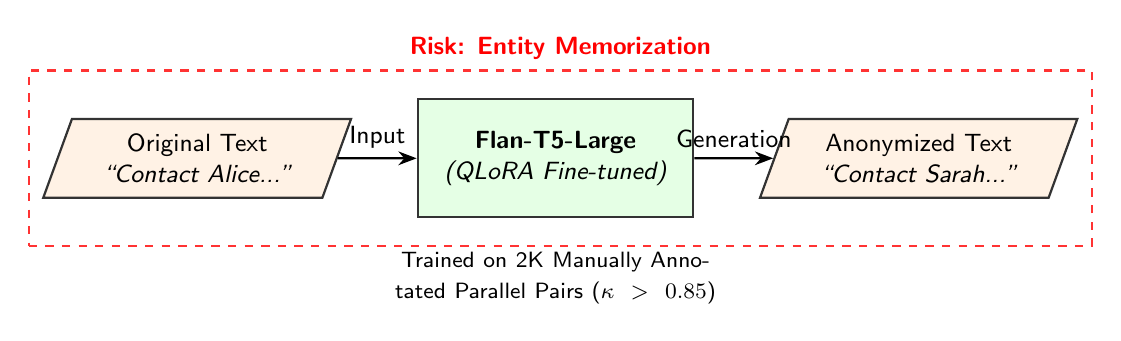
\begin{tikzpicture}[
    node distance=1.5cm and 1cm,
    font=\sffamily\small,
    thick,
    >=Stealth,
    process/.style={rectangle, draw=black!80, fill=blue!10, rounded corners, minimum width=3cm, minimum height=1.2cm, align=center},
    data/.style={trapezium, trapezium left angle=70, trapezium right angle=110, draw=black!80, fill=orange!10, minimum width=2.5cm, minimum height=1cm, align=center},
    model/.style={rectangle, draw=black!80, fill=green!10, minimum width=3.5cm, minimum height=1.5cm, align=center}
]
    \node[data] (input) {Original Text\\ \textit{``Contact Alice...''}};
    \node[model, right=of input] (t5) {\textbf{Flan-T5-Large}\\ \textit{(QLoRA Fine-tuned)}};
    \node[data, right=of t5] (output) {Anonymized Text\\ \textit{``Contact Sarah...''}};
    \node[draw=red!80, dashed, inner sep=10pt, fit=(input) (t5) (output)] (risk) {};
    \node[red, above] at (risk.north) {\textbf{Risk: Entity Memorization}};
    \draw[->] (input) -- node[above] {Input} (t5);
    \draw[->] (t5) -- node[above] {Generation} (output);
    \node[below=0.3cm of t5, align=center, text width=6cm] (note) {\footnotesize Trained on 2K Manually Annotated Parallel Pairs ($\kappa > 0.85$)};
\end{tikzpicture}%
}
\caption{Approach 1 (Baseline): Direct Seq2Seq on human-curated gold-standard pairs. High quality but susceptible to entity memorization.}
\label{fig:baseline}
\end{figure}

\textbf{Annotation Protocol:}
\begin{enumerate}
    \item Identify all PII spans (names, locations, organizations, dates, phone numbers).
    \item Replace with culturally and contextually plausible pseudonyms preserving entity type and demographic consistency.
    \item Rewrite pronouns and adjectives for grammatical agreement.
    \item Second annotator validates; disagreements resolved by consensus.
\end{enumerate}

\textbf{Training:} Fine-tune Flan-T5-Large (780M parameters) with QLoRA ($r{=}32$, $\alpha{=}64$) on this corpus:
\begin{equation}
    \mathcal{L}_{\text{baseline}} = -\sum_{i=1}^{N} \log P(x^{\text{anon}}_i \mid x^{\text{orig}}_{<i}, X_{\text{orig}})
\end{equation}

\subsection{Approach 2: Presidio + Rule-Based Baseline}

As a non-neural reference, we run Microsoft Presidio \cite{presidio2023} for entity detection, followed by type-aware random replacement from curated gazetteer lists (names from US Census, cities from GeoNames, organizations from Wikidata). This establishes the performance floor for contextual consistency.

\subsection{Approach 3: Zero-Shot LLM Anonymization}

We evaluate in-context anonymization by prompting an instruction-tuned LLM (Flan-T5-XL or a locally-hosted Mistral-7B-Instruct) with a structured prompt:
\begin{verbatim}
Anonymize the following text by replacing
all personal information with realistic
fictional alternatives. Maintain grammar
and meaning. Text: {input}
\end{verbatim}
This tests whether off-the-shelf LLMs can perform anonymization without task-specific training, providing a strong zero-shot baseline.

\subsection{Approach 4: DP-Guided Decoupled Mask-and-Fill (Ours)}

Our architecture eliminates privacy leakage through three complementary mechanisms.

\begin{figure}[ht]
\centering
\resizebox{\columnwidth}{!}{%
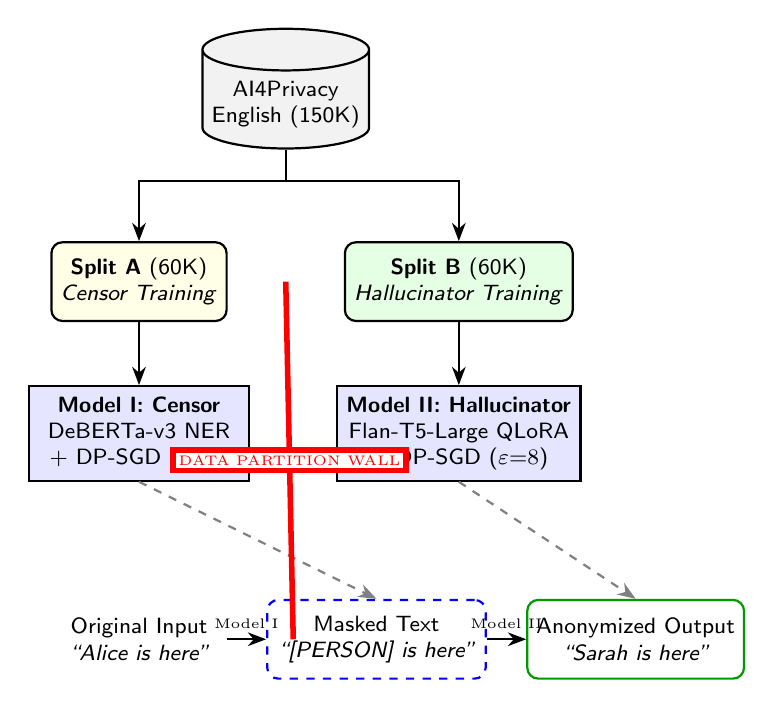
\begin{tikzpicture}[
    node distance=1.2cm and 0.5cm,
    font=\sffamily\footnotesize,
    thick,
    >=Stealth,
    process/.style={rectangle, draw=black, fill=white, rounded corners, minimum width=2.2cm, minimum height=1cm, align=center},
    database/.style={cylinder, shape border rotate=90, draw, fill=gray!10, aspect=0.25, minimum height=1.5cm, minimum width=1.5cm, align=center},
    model/.style={rectangle, draw=black, fill=blue!10, minimum width=2.8cm, minimum height=1.2cm, align=center},
    arrow/.style={->, thick}
]
    \node[database] (dataset) {AI4Privacy\\English (150K)};
    \node[process, below left=1.2cm and 0.2cm of dataset, fill=yellow!10] (splitA) {\textbf{Split A} (60K)\\ \textit{Censor Training}};
    \node[process, below right=1.2cm and 0.2cm of dataset, fill=green!10] (splitB) {\textbf{Split B} (60K)\\ \textit{Hallucinator Training}};
    \draw[arrow] (dataset.south) -- +(0,-0.4) -| (splitA.north);
    \draw[arrow] (dataset.south) -- +(0,-0.4) -| (splitB.north);
    \node[model, below=0.8cm of splitA] (model1) {\textbf{Model I: Censor}\\DeBERTa-v3 NER\\+ DP-SGD ($\varepsilon{=}8$)};
    \node[model, below=0.8cm of splitB] (model2) {\textbf{Model II: Hallucinator}\\Flan-T5-Large QLoRA\\+ DP-SGD ($\varepsilon{=}8$)};
    \draw[arrow] (splitA) -- (model1);
    \draw[arrow] (splitB) -- (model2);
    \node[coordinate, below=2cm of model1] (inference_start) {};
    \node[process, fill=white, draw=none] (input_text) at (inference_start) {Original Input\\ \textit{``Alice is here''}};
    \node[process, right=0.5cm of input_text, draw=blue, dashed] (masked_text) {Masked Text\\ \textit{``[PERSON] is here''}};
    \node[process, right=0.5cm of masked_text, draw=green!60!black, thick] (final_text) {Anonymized Output\\ \textit{``Sarah is here''}};
    \draw[arrow] (input_text) -- node[above, font=\tiny] {Model I} (masked_text);
    \draw[arrow] (masked_text) -- node[above, font=\tiny] {Model II} (final_text);
    \draw[->, dashed, gray] (model1.south) -- (masked_text.north);
    \draw[->, dashed, gray] (model2.south) -- (final_text.north);
    \draw[red, line width=2pt] ($(splitA.east)!0.5!(splitB.west)$) -- ($(model1.south east)!0.5!(model2.south west) + (0, -2)$) node[midway, fill=white, draw=red, inner sep=2pt, font=\tiny] {DATA PARTITION WALL};
\end{tikzpicture}%
}
\caption{DP-Guided Decoupled Pipeline (Approach 4). Models are trained on disjoint partitions with DP-SGD, and connected only through typed mask tokens at inference time.}
\label{fig:decoupled}
\end{figure}

\subsubsection{Mechanism 1: Disjoint Data Partitioning}
The English subset (after reserving 2K for Approach~1 and 10K for evaluation) is split:
\begin{itemize}
    \item \textbf{Split A} (60K): Trains Model~I (Censor) on (original $\rightarrow$ masked) pairs
    \item \textbf{Split B} (60K): Trains Model~II (Hallucinator) on (masked $\rightarrow$ pseudonymized) pairs
\end{itemize}
\textbf{Constraint:} $\text{Split A} \cap \text{Split B} = \emptyset$. The Hallucinator never sees original entities from the Censor's partition.

\subsubsection{Mechanism 2: DP-SGD Training}
Disjoint partitioning alone does not bound information leakage from pre-trained weights. We apply DP-SGD \cite{abadi2016deep} via Opacus \cite{opacus2021} to both models during fine-tuning:
\begin{equation}
    \tilde{g}_t = \frac{1}{B}\left(\sum_{i=1}^{B} \text{clip}(\nabla_\theta \mathcal{L}_i, C) + \mathcal{N}(0, \sigma^2 C^2 \mathbf{I})\right)
\end{equation}
where $C$ is the per-example gradient clipping norm, $\sigma$ is the noise multiplier, and the total privacy budget $(\varepsilon, \delta)$ is tracked via the RDP accountant. We target $\varepsilon \leq 8$ with $\delta = 1/N$.

\subsubsection{Model I: The Censor (Multi-Task DeBERTa-v3 NER)}
\textbf{Task:} High-recall PII detection via BIO token classification with learned privacy importance scoring.

\textbf{Architecture:} We introduce a \textbf{MultiTaskNERModel} built on DeBERTa-v3-small \cite{he2021debertav3} (44M params), jointly training two heads:
\begin{enumerate}
    \item \textbf{NER Classification Head}: Standard linear projection over BIO label space $C$, trained with recall-weighted focal loss ($\gamma{=}2, \alpha{=}0.25$).
    \item \textbf{Privacy Attention Head}: A multi-head attention layer (4 heads) over the token representations, followed by LayerNorm and a two-layer MLP with GELU activation and sigmoid output, producing per-token privacy importance scores $p_t \in [0,1]$. Supervised via BCE against entity masks (entity tokens$\rightarrow$1, O tokens$\rightarrow$0).
\end{enumerate}
The combined training objective is:
\begin{equation}
    \mathcal{L}_{\text{censor}} = \mathcal{L}_{\text{focal}} + \lambda_{\text{priv}} \cdot \mathcal{L}_{\text{privacy}}
\end{equation}
where $\mathcal{L}_{\text{focal}}$ is the focal loss over BIO labels, $\mathcal{L}_{\text{privacy}}$ is the BCE privacy attention loss, and $\lambda_{\text{priv}}{=}0.3$. The privacy attention head learns to assign high importance to tokens in sensitive contexts even before explicit entity classification, improving recall for ambiguous or rare entity types.

DP-SGD is applied via Opacus on a separate standard token classifier (to satisfy Opacus module constraints), with backbone weights transferred back to the multi-task model after training.

\subsubsection{Model II: The Hallucinator (Flan-T5-Base + QLoRA + Semantic Fidelity Loss)}
\textbf{Task:} Generate contextually consistent pseudonyms from masked templates while preserving semantic content.

\textbf{Training:} Fine-tune Flan-T5-Base (250M params) with QLoRA ($r{=}16$, $\alpha{=}32$, 4-bit NF4 quantisation) on Split~B:
\begin{itemize}
    \item Input: \texttt{``Fill PII: [PERSON] works at [ORG] in [LOC]''}
    \item Target: \texttt{``Jessica works at NovaCorp in Portland''}
\end{itemize}

\textbf{BERTScore-Inspired Semantic Fidelity Loss:} Beyond standard cross-entropy, we introduce a \textit{semantic fidelity regulariser} inspired by BERTScore \cite{zhang2020bertscore}. During training, we extract encoder and decoder hidden states, mean-pool them (using attention masks), and compute their cosine similarity. The loss penalises deviations from a target similarity $\tau{=}0.70$:
\begin{equation}
    \mathcal{L}_{\text{halluc}} = \mathcal{L}_{\text{CE}} + \lambda_{\text{sem}} \cdot \text{MSE}\!\left(\cos(\bar{h}_{\text{enc}}, \bar{h}_{\text{dec}}),\; \tau\right)
\end{equation}
where $\bar{h}_{\text{enc}} = \text{MeanPool}(H_{\text{enc}}, M_{\text{attn}})$, $\bar{h}_{\text{dec}} = \text{MeanPool}(H_{\text{dec}}, M_{\text{label}})$, and $\lambda_{\text{sem}}{=}0.15$. This encourages the model to preserve the semantic structure of the input while replacing entities, avoiding degenerate outputs that merely copy or hallucinate unrelated content.

\textbf{Key Property:} Model~II learns $P(X_{\text{anon}} \mid X_{\text{mask}})$ conditioned \textit{only} on mask templates. Combined with DP-SGD, the information any single training example can contribute is bounded by $\varepsilon$.

\subsubsection{Mechanism 3: Entity Consistency Module}
A critical limitation of independent fill-in-the-blank generation is \textit{entity inconsistency}: the same masked entity ``[PERSON]'' in different sentences may receive different pseudonyms. We address this with a deterministic consistency layer:
\begin{enumerate}
    \item Extract all masked spans with their surrounding context windows ($\pm$10 tokens).
    \item Compute a \texttt{SHA-256} hash of (entity\_type, context\_signature) to produce a deterministic seed.
    \item Use this seed to select from Model~II's top-$k$ candidates, ensuring the same entity-in-context always maps to the same pseudonym within a document.
\end{enumerate}
This maintains co-reference coherence (``Alice'' $\rightarrow$ ``Sarah'' everywhere in a document) without storing any mapping between original and synthetic entities.

\subsubsection{Inference Pipeline}
\begin{enumerate}
    \item Input original text $X_{\text{orig}}$
    \item Model~I: $X_{\text{orig}} \xrightarrow{\text{Censor}} X_{\text{mask}}$ (PII detection + typed masking)
    \item Entity Consistency: Group co-referent masks by (type, context hash)
    \item Model~II: $X_{\text{mask}} \xrightarrow{\text{Hallucinator}} X_{\text{anon}}$ (contextual pseudonym generation)
    \item Consistency enforcement: Identical hashes $\rightarrow$ identical pseudonyms
    \item Output anonymized text $X_{\text{anon}}$
\end{enumerate}

\section{Evaluation Plan}
We curate a held-out test set (10K instances) with stratified entity type distribution and manual verification.

\subsection{Privacy Metrics}
\begin{itemize}
    \item \textbf{Entity Leakage Rate (ELR)}: Exact-match and fuzzy-match (Levenshtein $\leq 2$) percentage of original entities appearing in anonymized output.
    \item \textbf{Membership Inference Attack (MIA)}: Train a shadow-model adversary \cite{shokri2017membership} and report attack AUC; lower is better (random = 0.5).
    \item \textbf{Entity Re-identification via Embedding Similarity}: Compute cosine similarity between SBERT embeddings of original and anonymized entities; measure top-$k$ retrieval accuracy.
    \item \textbf{Formal $(\varepsilon, \delta)$ Budget}: Report the actual consumed privacy budget from Opacus RDP accountant.
\end{itemize}

\subsection{Utility Metrics}
\begin{itemize}
    \item \textbf{Linguistic Quality}: BLEU, METEOR, BERTScore against reference anonymizations.
    \item \textbf{Masking Quality (Censor-Specific)}: BLEU, ROUGE-L, and token accuracy evaluated on the NER masking step \textit{in isolation}, enabling fine-grained diagnosis of privacy detection independently from hallucination quality.
    \item \textbf{Grammatical Correctness}: LanguageTool error rate + human evaluation (3 annotators, Likert 1--5).
    \item \textbf{Entity Consistency Score}: Percentage of co-referent entities receiving identical pseudonyms within a document.
    \item \textbf{Semantic Preservation}: Sentence-BERT cosine similarity between original and anonymized non-entity context.
\end{itemize}

\subsection{Downstream Task Performance}
\begin{itemize}
    \item \textbf{Sentiment Analysis}: Fine-tune RoBERTa-base on anonymized vs.\ original SST-2; compare accuracy.
    \item \textbf{Named Entity Recognition}: Train NER on anonymized CoNLL-2003, test on original; report F1.
    \item \textbf{Text Classification}: Compare F1 on AG News anonymized corpus.
    \item \textbf{Question Answering}: Fine-tune on anonymized SQuAD 2.0; report EM and F1.
\end{itemize}

\subsection{Ablation Studies}
\begin{itemize}
    \item Effect of DP noise multiplier $\sigma \in \{0.5, 1.0, 1.5, 2.0\}$ on privacy-utility tradeoff.
    \item With vs.\ without entity consistency module.
    \item Data partition ratio (50/50 vs.\ 70/30 vs.\ 90/10) impact on both models.
    \item QLoRA rank $r \in \{8, 16, 32, 64\}$ ablation.
    \item \textbf{Privacy Attention Head}: Multi-task NER with vs.\ without learned privacy importance scores.
    \item \textbf{Semantic Fidelity Loss}: Training with vs.\ without the BERTScore-inspired semantic regulariser; varying target similarity $\tau \in \{0.5, 0.7, 0.9\}$.
    \item \textbf{Model Efficiency}: DeBERTa-v3-small (44M) vs.\ DeBERTa-v3-base (184M) for NER; Flan-T5-small (77M) vs.\ Flan-T5-base (250M) for generation --- measuring Pareto-optimal accuracy-per-FLOP frontier.
\end{itemize}

\section{Expected Outcomes and Timeline}

\subsection{Research Questions}
\begin{enumerate}
    \item \textbf{RQ1}: Does DP-SGD + disjoint partitioning provide measurably stronger privacy guarantees than partitioning alone, and at what utility cost?
    \item \textbf{RQ2}: How does the four-way comparison (human-curated, Presidio, zero-shot LLM, decoupled DP) rank on the privacy-utility Pareto frontier?
    \item \textbf{RQ3}: Does the entity consistency module improve downstream task performance without degrading privacy?
    \item \textbf{RQ4}: What is the optimal $(\varepsilon, r, \text{partition ratio})$ configuration for production deployment?
\end{enumerate}

\subsection{Tentative Timeline}
\begin{table}[ht]
\centering
\small
\begin{tabular}{@{}ll@{}}
\toprule
\textbf{Milestone} & \textbf{Deadline} \\
\midrule
Dataset preparation, partitioning, annotation & Week 1 \\
Baseline training (Human-curated + Presidio) & Week 2 \\
Model I (Censor DeBERTa) + DP-SGD training & Week 3 \\
Model II (Hallucinator Flan-T5) + QLoRA & Week 4 \\
\textbf{Interim Report \& Preliminary Results} & \textbf{Week 5} \\
Evaluation pipeline + adversarial attacks & Week 6 \\
Ablations + human evaluation & Week 7 \\
\textbf{Final Report \& Presentation} & \textbf{Week 8} \\
\bottomrule
\end{tabular}
\caption{Project execution timeline (8-week schedule).}
\label{tab:timeline}
\end{table}

\subsection{Potential Challenges}
\begin{itemize}
    \item \textbf{DP-Utility Tradeoff}: Aggressive noise may degrade generation quality; we ablate $\sigma$ to find the Pareto-optimal point.
    \item \textbf{Cascade Errors}: Censor misses propagate to Hallucinator; we measure recall at each stage and analyze error composition.
    \item \textbf{Entity Type Imbalance}: Rare types (SSN, IBAN) may be under-represented; we apply stratified sampling and report per-type metrics.
    \item \textbf{Computational Cost}: DP-SGD increases per-step cost 2--3$\times$; QLoRA and gradient checkpointing mitigate this.
\end{itemize}

\section{Conclusion}
This project addresses a critical gap in privacy-preserving NLP by combining disjoint data partitioning with formal differential privacy guarantees --- going beyond the common but ungrounded assumption that data separation alone prevents leakage. Through a four-way comparison spanning human-curated, rule-based, zero-shot LLM, and our DP-guided decoupled architecture, we provide rigorous empirical evidence on the privacy-utility Pareto frontier. The entity consistency module ensures practical usability for document-level anonymization. Our findings inform the design of production-ready, regulation-compliant anonymization pipelines.

\bibliographystyle{plain}
\bibliography{references}

\end{document}